\documentclass{article}
\usepackage{listings}
\usepackage{graphicx}
\graphicspath{ {/} }
\begin{document}
\begin{titlepage}
\centering

{\bfseries\LARGE Instituto Polit\'ecnico Nacional \par}
\vspace{1cm}
{\scshape\Large Escuela Superiror de Computaci\'on \par}
\vspace{3cm}
{\scshape\Large Teoria de la Computaci\'on \par}
\vspace{3cm}
{\itshape\Large Pr\'actica 3 \par}
{\itshape\Large Protocolo \par}
\vfill
{\Large Profesor: \par}
{\Large Genaro Juarez Martinez \par}
{\Large Alumno: \par}
{\Large Alcantara Covarrubias Erik \par}
{\Large Email: erik.alcova@gmail.com \par}
{\Large Grupo: 4SCM6\par}
\vfill
\end{titlepage}

\tableofcontents

\newpage

\section{Introducción}
Los autómatas finitos usan ”lenguajes” con reconocimiento de tres tipos, gramáticas regulares, autómatas finitos o expresiones regulares.
\\Los autómatas finitos tienen un cojunto de estados y su control pasa de un estado a otro dependiendo de las
entradas externas. 
\\Una caracteristica de los autómatas deterministicos es que no se puede estar en dos estados a
un mismo tiempo.
\\Los autómatas tienen representaciones graficas que nos ayudan a poder entender como se dan los cambios de estado o también se
pueden ver por medio de una tabla.

\section{Marco Teorico}

    Nota: 
    \\Lenguaje ($\sum$): Conjunto de simbolos que conforman un alfabeto
    \\$\sum = \{ 0, 1\}$ Es un lenguaje conformado por el 0 y el 1.
    \\$\sum = \{A, ..., Z\}$ Es un lenguaje conformado por las letras arabigas.\\
    
    Un autómata finito deterministico es aquel que solo puede estar en un único estado después de leer cualquier
    secuencia de entradas. Este autómata finito deterministico está constituido por:
\begin{enumerate}
    \item Un conjunto finito de estados Q. 
    \item Un conjuto finito de simbolos de entrada
\end{enumerate}
    Una función de transición la cual toma un argumento y un elemento y regresa un estado, esta función es designada por $\delta$ mientras que en el tema de los grafos se designa por circulos y etiquetas que demuestran los estados.
\begin{enumerate}
    \item Un estado inicial, el cual es uno de los estados Q.
    \item Un $\delta$ (diferencia) conjunto de estados finales o de aceptación F tomando en cuenta que $F \subseteq  Q$.
\end{enumerate}
    
    Usando la notación ”quintupla” se denota al autómata finito deterministico como:
\begin{center}
    $A = \{Q, \delta , q0 , F \}$
\end{center}
    
\section{Desarrollo}
El Algoritmo es sencillo en concepcion, es generar $10^6$ cadenas binarias y que el automata lo "limpie" y determine si es par o no.

\subsection{Programa 3 - Protocolo}
Realiza un program que simule el funcionamiento de un protocolo utilizando un AFD\begin{enumerate}
    \item El programa debe funcionar automaticamente.
    \item Debe de verificar si el protocolo está encendido o apagado y ejecutarse nuevamente si está encendido. 
    \\El programa deberá determinar automáticamente para detenerse.
    \item Generara $10^6$ cadenas binarias aleatoriamente de longitud de 64 bits.
    \item Hacer que el programa se espere 1 segundo
    \item Posteriormente calidar cada una de las cadenas con el AFD de paridad
    \item Generar cuatro archivos de texto para las salidas
    \item Tener la opción de graficar el AFD completo (protocolo y paridad en el mismo grafo)
\end{enumerate} 

\subsection{Codigo}

\begin{lstlisting}
import random
import time
import graphviz 
import tempfile

def grafica():
  f = graphviz.Digraph('finite_state_machine')
  f.attr(rankdir='LR')

  f.attr('node', shape='doublecircle')
  f.node('Q0')
  f.node('Inicio')

  f.attr('node', shape='plaintext')
  f.edge('', 'Q0', label='Inicio')

  f.attr('node', shape='circle')
  f.edge('Inicio', 'Inicio', label='Apagado')
  f.edge('Inicio', 'Listo', label='Encendido')
  f.edge('Listo', 'Q0', label='Cadena')
  f.edge('Enviar', 'Listo')
  f.edge('Enviar', 'Enviar', label='Espera de 1s')
  f.edge('Listo', 'Inicio' ,label='Despues de 10^6 cadenas')
  f.edge('Q0', 'Enviar', label='Nueva cadena')
  f.edge('Q0', 'Q2', label='1')
  f.edge('Q0', 'Q1', label='0')
  f.edge('Q2', 'Q0', label='1')
  f.edge('Q1', 'Q0', label='0')
  f.edge('Q1', 'Q3', label='1')
  f.edge('Q3', 'Q1', label='1')
  f.edge('Q2', 'Q3', label='0')
  f.edge('Q3', 'Q2', label='0')
  f.view(tempfile.mktemp())

def par(num):
  if num % 2 == 0:
    return True
  else:
    return False

def repre_adf(pre, simbolo, arch):
    if(pre == "q0"):
        if(simbolo == "1"):
            siguiente = "q2"
        else:
            siguiente = "q1"
    elif(pre == "q1"):
        if(simbolo == "1"):
            siguiente = "q3"
        else:
            siguiente = "q0"
    elif(pre == "q2"):
        if(simbolo == "1"):
            siguiente = "q0"
        else:
            siguiente = "q3"
    elif(pre == "q3"):
        if(simbolo == "1"):
            siguiente = "q1"
        else:
            siguiente = "q2"
    arch.write("| f("+pre+", "+simbolo+") -> "+siguiente+" |")
    return siguiente

def binario_random(n):
    anterior = "q0"
    
    filelog = open("Practica3/Automata.txt", "a+")
    key1 = ""
    
    for i in range(n):
         
        temp = str(random.randint(0, 1))
        anterior = repre_adf(anterior, temp, filelog)
        key1 += temp
    
    filelog.write("\n")
    filelog.close()
    return key1

def transformar(num):
  unos = 0
  global aceptados
  global rechazados
  
  for i in num:
    unos += int(i)
  ceros = len(num) - unos
  return unos, ceros
  
def adf(array, num, acep, rec):
  
  num.write(array+"\n")
  unos, ceros = transformar(array)
  
  if(par(unos) and par(ceros)):
    acep.write(array+"\n")
  else:
    rec.write(array+"\n")
  
def new_gen():
  
  filenum = open("Practica3/Numeros.txt", "w")
  fileace = open("Practica3/Aceptados.txt", "w")
  filerec = open("Practica3/Rechazados.txt", "w")
  
  num = []
  inicio = time.time()  
  
  for i in range(10**6): #(10**6)
    try:
      task = binario_random(64) #64
      num.append(task)
      del task
          
    except (KeyboardInterrupt, OverflowError):
      break
    
  fin = time.time()
  
  print("El tiempo de ejecucion de generacion de cadenas es: "+str(fin-inicio))
  print("Inicia el ADF")
  
  for i in num:
    adf(i, filenum, fileace, filerec)
  return num

  filenum.close() 
  fileace.close() 
  filerec.close() 
  
def protocolo():
  repeticiones = 0
  while(bool(random.getrandbits(1))):
    estado = bool(random.getrandbits(1))
    filelog = open("Practica3/Automata.txt", "w")
    filelog.close()
      
    if(estado):
      numeros=new_gen()
      time.sleep(1)
      print("Total cadenas:"+str(len(numeros)))
      del numeros
    else:
      print(estado)
    repeticiones += 1
    
  print("El programa se ejecuto: "+str(repeticiones)+" veces")
  
if __name__ == "__main__":
    """Main function"""
    
    print("Practica #3")
    
    while(True): 
      print("1) Ejecutar programa")
      print("2) Graficar Automata")
      print("3) Salir")
      opc = int(input("Selecciona la opcion: "))
      if(opc == 1):
        protocolo()
      
      elif(opc == 2):
        grafica()
      
      elif(opc == 3):
        exit()
      
      else:
        print("Opcion no valida, porfavor introduzca una opcion correcta")
\end{lstlisting}

\section{Resultados}

Esta es la grafica que aparece al darle la opcion 2 del menu:
\begin{center}
    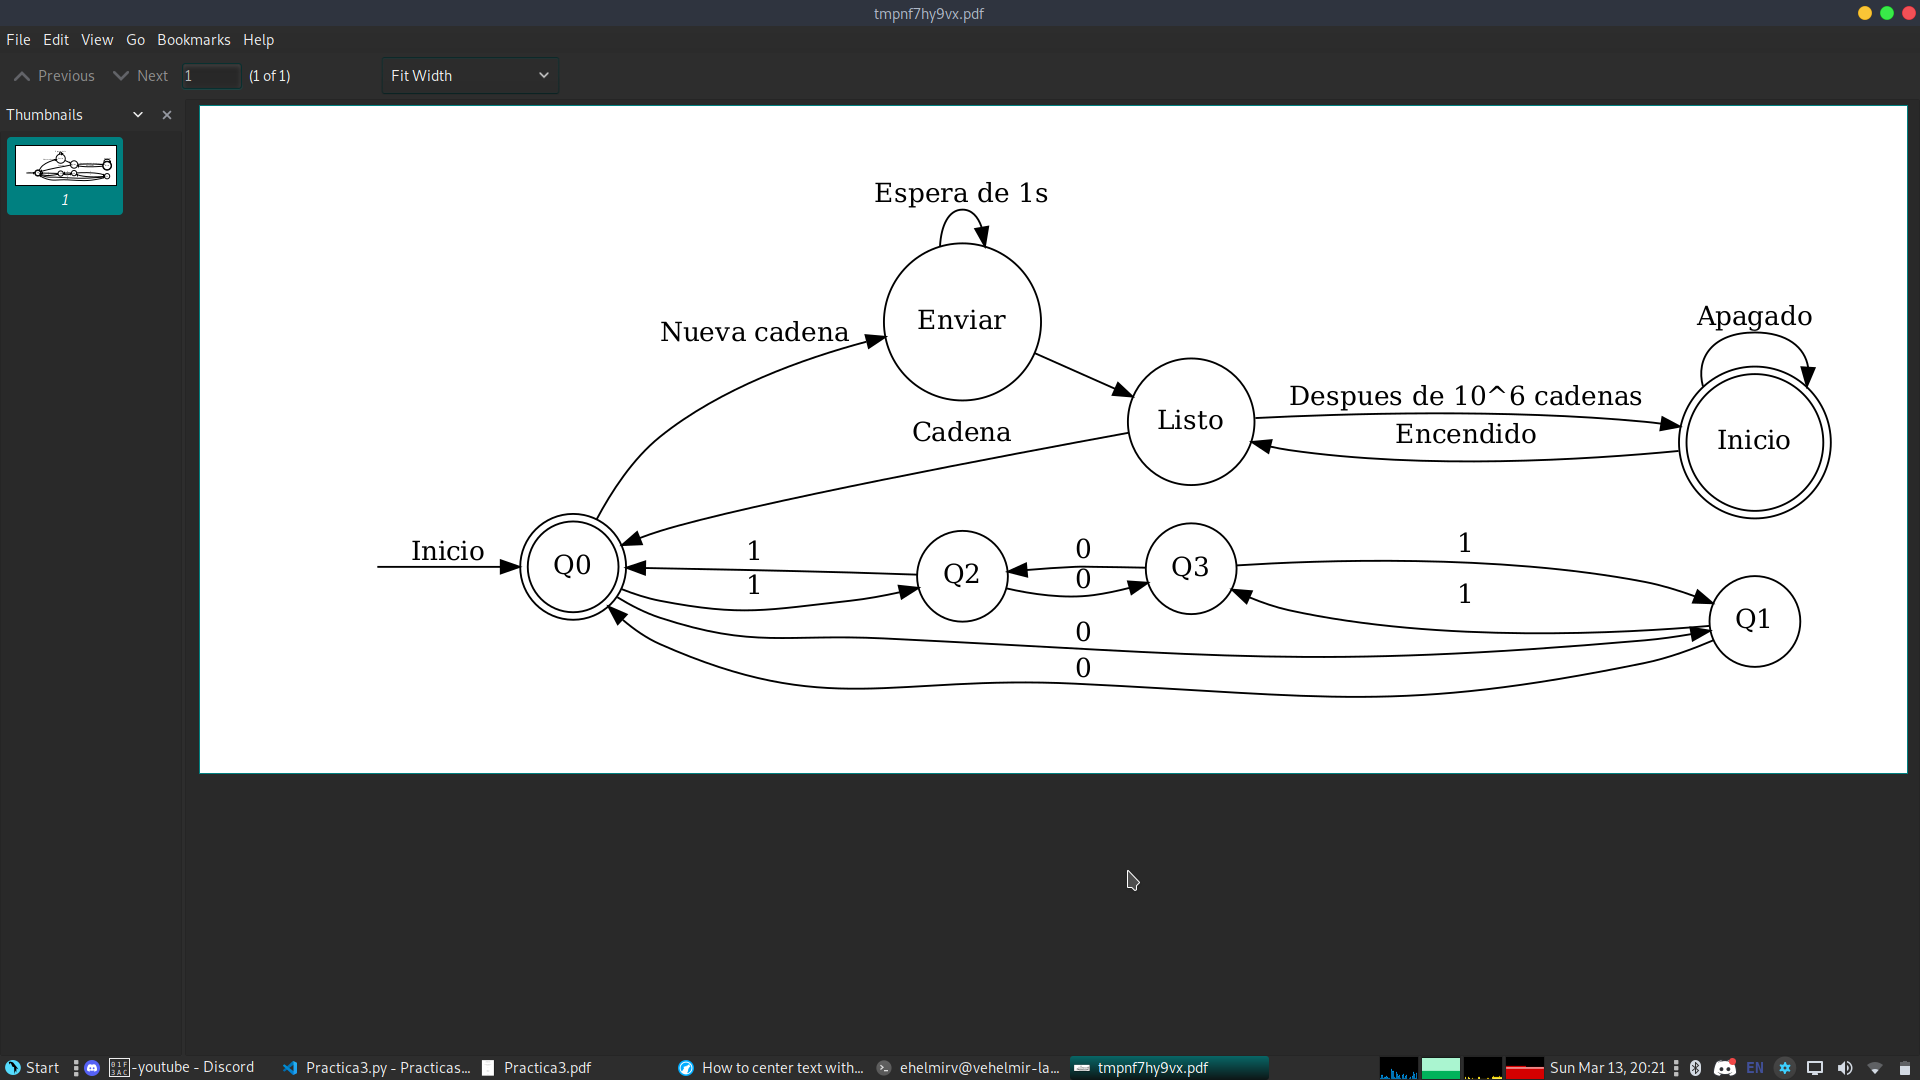
\includegraphics[width=\textwidth]{Grafica.png}
\end{center}
Se crean 4 archivos .txt:
\begin{itemize}
    \item Numeros: Que muestra todos los numeros generados.
    \item Aceptados: Las cadenas que acepta el AFD.
    \item Rechazados: Todas las cadenas que no acepta el ADF.
    \item Automata: Que movimientos hace el automata para reconocer la cadena.
\end{itemize}

\section{Conclusión}
El Algoritmo fue sencillo de realizar y la optimizacion fue sencilla gracias al uso de un adf, por lo que en su mayoria al adf se encargaba de todo.
\\Al poder definir visualmente el como iba a comportarse el adf fue sencilo extrapolarlo a codigo del mundo real lo que ayudo enormemente.
\\En conclusion; los ADF facilitan mucho la creacion de codigo facil de entender y de mantener en un ambiente laboral.

\section{Referencias bibliograficas}
\begin{itemize}
    \item LaTeX - A document preparation system. (s. f.). LaTeX - A document preparation system. https://www.latex-project.org/
\end{itemize}
\end{document}